\documentclass[a5paper]{article}
\usepackage[utf8]{inputenc}
\usepackage[T1]{fontenc}
\usepackage{txfonts}
\usepackage{bm}
\usepackage{geometry}
\usepackage{graphics}

\title{Statistics}
\author{Jon Hurst}

\begin{document}
\maketitle

\section{Mean, Variance and Standard Deviation}

If $f_i$ is the frequency that value $x_i$ occurs and $\overline{x}$ and
$\sigma^2$ are respectively the mean and variance for the frequency
distribution, then

\begin{equation}
  \overline{x} = \frac{\sum\limits_{all\ i} f_i x_i}{\sum\limits_{all\ i} f_i}
\end{equation}

\begin{equation} \label{eq:1}
  \sigma^2 = \frac{\sum\limits_{all\ i} f_i (x_i - \overline{x})^2}{\sum\limits_{all\ i} f_i}
\end{equation}

Since

\begin{equation}
  \frac{\sum\limits_{all\ i} f_i (x_i - \overline{x})^2}{\sum\limits_{all\ i} f_i} =
  \frac{\sum\limits_{all\ i} f_i x_i^2}{\sum\limits_{all\ i} f_i}
  -2\overline{x}\ \frac{\sum\limits_{all\ i} f_i x_i}{\sum\limits_{all\ i} f_i}
  + \overline{x}\ \frac{\sum\limits_{all\ i} f_i}{\sum\limits_{all\ i} f_i}
\end{equation}

An alternative version of (\ref{eq:1}) is

\begin{equation} \label{eq:2}
  \sigma^2 = \frac{\sum\limits_{all\ i} f_i x_i^2}{\sum\limits_{all\ i} f_i} -
  \overline{x}^2
\end{equation}

(\ref{eq:2}) is sometimes verbalised as ``the mean of the squares minus the square
of the means''.

Standard deviation, $\sigma$, is the square root of the variance. The advantage
of the standard deviation is that it has the same units as the mean.

\section{Weighted Mean}

The concept of a weighted mean is that some values are considered to be ``more
important'' to the mean than others. If we had, for example, a set of integer
values between 1 and 10 and we wanted 7 to be twice as important to the mean as
the other numbers, if each time 7 occurs we treat it as having occurred twice we
achieve the desired effect. In general, if we assign a weight, $w_i$, to each
possible value, then

\begin{equation}
  \overline{x} = \frac{\sum\limits_{all\ i} w_i f_i x_i}{\sum\limits_{all\ i}
    w_i f_i}
\end{equation}

Considering the above example, $w_i$ could be $1$ except for $w_7$ which would
be $2$. If $w_i$ were $\frac{1}{11}$ except for $w_7$ which would be
$\frac{2}{11}$, the result is the same because the $\frac{1}{11}$ factor can be
taken outside the summation signs for both numerator and denominator. The latter
scheme allows the total weight to add to 1, which is often how weights are
specified.

\section{Arrangements}

Consider all the ways that the numbers in the set \{1,2,3,4\} could be ordered.
One way to do this methodically would be with a tree diagram, as shown if Figure
\ref{fig:1}. The total number of possible arrangements is the number of entries
on the bottom line, and this can be seen to be $4\times 3\times 2\times 1 = 24$.
Essentially, there are 4 ways to fill the first number, then for each of those
4, 3 ways to fill the second number, then for each of those 3 only 2 ways to
fill the third number, with the last number being the only one remaining.

\begin{figure}[ht]

  \begin{center}
    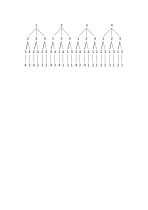
\includegraphics{arrangements}
  \end{center}
  \caption{Arrangements tree}
  \label{fig:1}
\end{figure}

This process can be generalised for $n$ numbers. The number of arrangements of
$n$ numbers will result from there being $n$ ways to fill the first number, then
for each of those $n$ ways, $(n-1)$ ways to fill the second number, continuing
until there is only one option for the final number. If $A_n$ is the number of
possible arrangements of $n$ numbers, therefore

\begin{equation}
  A_n = n!
\end{equation}

These numbers can, of course, represent any set of $n$ distinct objects -- you
could always write the numbers on a sticky label and attach them to the objects.

\begin{figure}[ht]
  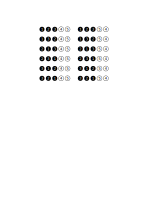
\includegraphics{arrangement-grouping}
  \caption{Arrangement grouping}
  \label{fig:2}
\end{figure}

A question that does, however, arise, is what happens if some of the objects are
identical, e.g. how many arrangements can be made of 3 black balls and 2 white
balls, given that you can't tell the difference between balls of the same
colour? The trick here is to label them first, so that you \textit{can} tell the
difference, then group the results together that would be indistinguishable
without the labels. In this example there are $5!$ ways of arranging the
labelled balls, and each grouping includes the $3!$ ways the black balls could
be arranged and the $2!$ ways the white balls could be arranged that would
result in indistinguishable results (see Figure \ref{fig:2}). Thus each group
contains $3!2! = 12$ results, meaning that there are $5!/12 = 10$
distinguishable arrangements.



\section{Permutations and Combinations}

If were to write down all the ways that two numbers can be randomly selected from
the set \{1, 2, 3, 4, 5\}, working methodically we would write \{1,2\}, \{1,3\},
\{1,4\}, \{1,5\}, \{2,1\}, \{2,3\} \ldots. Since there are 5 ways of filling the
first number, and then 4 ways of filling the second number for each of those
5 ways, there are a total of 20 possible results.

Generalising, if ${}^nP_r$ is the number of possible results from selecting $r$
objects from a set of $n$ objects, a.k.a. the number of permutations,

\begin{equation}
  {}^nP_r = \frac{n!}{(n-r)!}
\end{equation}

If, in the original example, we wanted to consider \{1,2\} and \{2,1\} to be the
same result, i.e. we did not consider order to be important, we can split the
original permutations up into groups where the results are considered to be the
same. In this case, the size of each group is 2, so there are 10 possible
results.

In general, if we select $r$ objects from $n$ objects and then group them on the
basis that order is unimportant, each group will be $r!$ in size since there are
$r!$ ways of arranging $r$ objects. If, then, ${}^nC_r$ is the number of
possible results from selecting $r$ objects from a set of $n$ objects if order
is considered unimportant, a.k.a. the number of combinations

\begin{equation}
  {}^nC_r = \frac{{}^nP_r}{r!} = \frac{n!}{(n-r)!r!}
\end{equation}

The trick of grouping permutations that are considered to be the same result
also works for rings. In a ring of $r$ objects where rotation is considered
unimportant, the size of the permutation groups will be $r$, since there are $r$
rotations of the ring that are considered to be the same result. If the ring can
also be flipped, that doubles the number of permutations considered to be the
same result, so size of each permutation group is $2r$.
\end{document}
